\chapter{Objektidentifiering}
\label{objektidentifiering}
Vid fjärrarbete kan det vara svårt för användaren att veta med vilka krafter robothanden påverkar objekt. För att underlätta detta implementeras en objektidentifieringsfunktion i robothanden som kan särskilja förinställda objekt. Dessa objekt kan lagras i robothandens dataminne tillsammans med största tillåtna tryck robothanden får lov att applicera på objektet. Denna information används för att begränsa kontakttrycket för respektive objekt och därmed riskerar användaren inte att skada objektet eller arbeta med onödigt höga krafter. 
\section{Identifieringsprincip}
Objektidentifieringen bygger på att robothanden beräknar avståndet mellan finger 1 och tummen vid trycksensorerna,se~\ref{fig:objektid} nedan. Varje objekt har ett identifierande mått. Detta betyder att objekt som skall särskiljas inte kan ha detta mått gemensamt.


\begin{figure}[H]
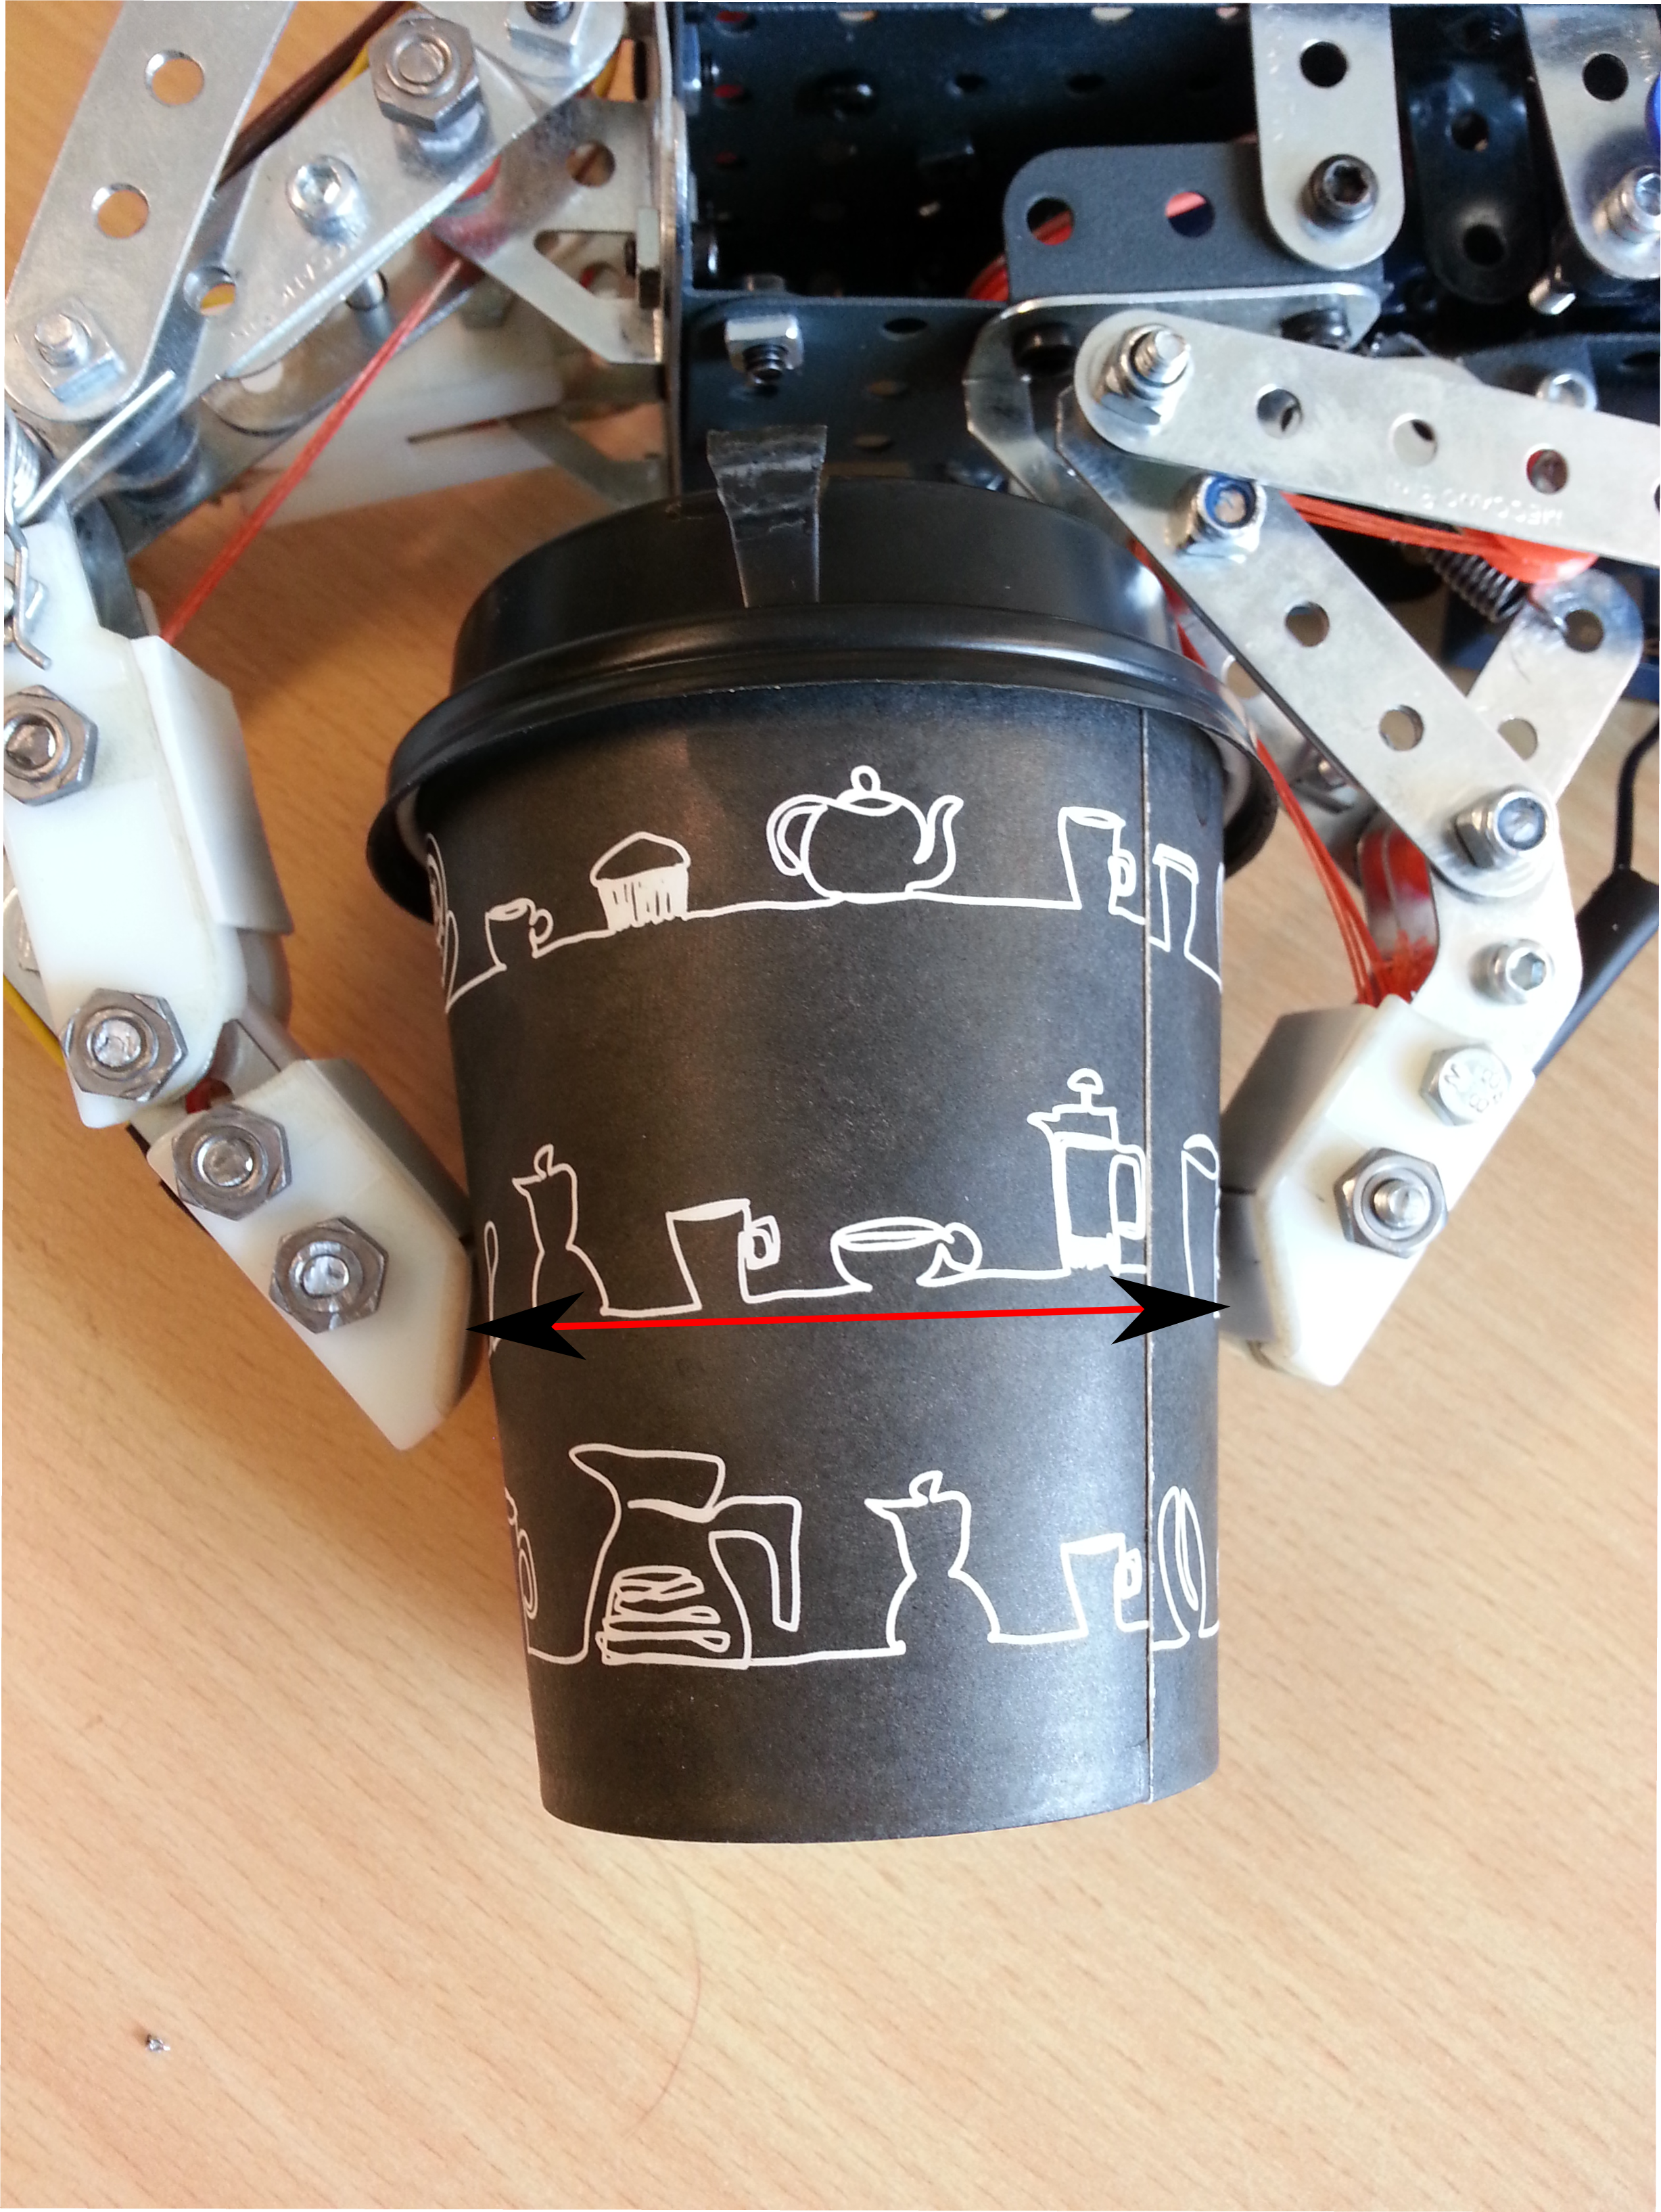
\includegraphics{img/obj_dist}
\caption{Identifiering av objekt}
\label{fig:objektid}
\end{figure}

För att beräkna avståndet mellan fingertopparna har en matematisk modell av handen tagits fram. Den utgår från servomotorernas önskade vridningsvinklar för att bestämma hur fingrarna är ställda. Då ingen mätning av servomotorernas faktiska läge görs finns endast information om den önskade vinkeln, men då servomotorerna reglerar sig själva kommer de efter en viss tidsfördröjning nå dit, förutsatt att de inte blir behindrade. Denna tidsfördröjning försummas då den är liten vid de små manipulationer av robothanden som görs då användaren försöker gripa ett objekt. Totalt är det fyra servomotorer som inverkar på avståndet mellan fingertopparna. Modellen baseras på vridningsvinklarna ($\varphi_1$,$\varphi_2$,$\varphi_3$,$\varphi_4$) som är de servolägen som entydigt bestämmer avståndet mellan fingertopparna. 

\begin{figure}[H]
\includegraphics[width=\textwidth]{img/obj_id_matlab}
\caption{plot över fingrets rörelse från den matematiska modellen}
\label{fig:objektidentifiering2}
\end{figure}
En fullständig matematisk modell av finger 1 och tummen tas fram och demonstreras med hjälp av matlab i figur~\ref{fig:objektidentifiering2} ovan. För fullständig beräkningsgång för att Appendix~\ref{servoberakningar}.


Objektidentifieringen har ett genomsnittligt fel på 20\%. Felet varierar beroende på i vilket område fingrarns befinner sig i. Arbetsområdet rekonmenderas att ligga mellan 40-100 mm där en upplösning på 15 mm erhålles. Figur \ref{fig:verk_berak} jämför uppmätta värden med de värden framtagna med hjälp av den mattematiska modellen. För att få en ökad precision rekomenderas att de felkällor som tas upp i \ref{felkallor} åtgärdas. Figur \ref{fig:objektidentifiering2} visualiserar handens rörelse med hjälp av den mattematiska modellen.

\begin{figure}[H]
\includegraphics[width=0.8\textwidth]{img/obj_id_matlab2}
\caption{plot över det uppmätta avstånden jämfört med det uträknade}
\label{fig:verk_berak}
\end{figure}




\subsubsection{Felkällor}
\label{felkallor}
Objektidentifieringen inehåller främst två felkällor som bidrar till en minskad precision. En av felkällorna är att modellen är baserat på önskade servolägen, dvs de lägen som specificerats av användaren. Om servomotorerna möter på motstånd som förhindrar rörelse till önskat läge kommer det faktiska avståndet och det avstånd beräknat genom modellen att skillja vilket bidrar till ett fel. Bild \ref{fig:objident1}-\ref{fig:objident2} illutrerar en situation då detta fel inträffar.

\begin{figure}[H]

        \begin{subfigure}[b]{0.5\textwidth}
                \centering
                \includegraphics{img/grepp}
                \caption{Faktiskt servoläge}
                \label{fig:objident1}
        \end{subfigure}%
       ~
        \begin{subfigure}[b]{0.5\textwidth}

                \includegraphics{img/grepp_verk}
                \caption{Önskat servoläge}
                \label{fig:objident2}
        \end{subfigure}

\end{figure}

För att lösa detta problem behöver systemet få information om handens faktiska läge. Detta kan åstadkommas genom att ansluta vinkelgivare till fingrets leder alternativt till servomotorerna. \

En annan stor felkälla är att handens konstruktion bidrar med låg precision, pga det mekaniska glappet. Mekanots låga toleranser gör att ett givet servoläge kan innebära många olika positioner. Felkällans magnitud ökar fort med ett ökat antal leder. För att öka precisionen behövs konstruktionen ändras för att exkludera det mekaniska glappet.
